\section{Hierarcha i opis funkcji modułów}
\label{sec:hierarchia}

Projekt składa się z ośmiu modułów, których hierarchia przedstawiona jest na
poniższym drzewie:
\begin{itemize}
  \item \texttt{mouse\_test.sch}
    \begin{itemize}
      \item \texttt{main.sch}
        \begin{itemize}
          \item \texttt{driver.vhd}
          \item \texttt{ps2\_rx.vhd}
          \item \texttt{ps2\_tx.vhd}
        \end{itemize}
      \item \texttt{controller.vhd}
      \item \texttt{vga.vhd}
      \item \texttt{RAM.xco}
    \end{itemize}
\end{itemize}
\vspace{1em}

\texttt{RAM.xco} to moduł dwuportowej pamięci RAM adresowanej bitowo z
magistralą adresową o szerokości 16 bitów. Moduł został wygenerowane za pomocą
narzędzia Xilinx Core Generator.

\subsection{Moduł \texttt{mouse\_test.sch}}
Jest to główny moduł projektu. Zawiera podmoduły odpowiedzialne za obsługę myszy
oraz ekranu oraz kontroler interpretujący dane przychodzące z modułu myszy.
Schemat modułu znajduje się na rysunku~\ref{fig:main}.
\vspace{1em}

Wejścia:
\begin{itemize}
  \item \texttt{clk} -- zegar 50MHz
  \item \texttt{rst} -- reset układu
\end{itemize}
\vspace{1em}
Wyjścia:
\begin{itemize}
  \item \texttt{vga\_vs} -- sygnał synchronizacji pionowej VGA
  \item \texttt{vga\_hs} -- sygnał synchronizacji poziomej VGA
  \item \texttt{vga\_c(2:0)} -- magistrala przesyłająca bity koloru do VGA
\end{itemize}
\vspace{1em}
Wyjścia dwukierunkowe:
\begin{itemize}
  \item \texttt{ps2\_data} -- linia danych PS/2
  \item \texttt{ps2\_clock} -- linia zegara PS/2
\end{itemize}

\subsection{Moduł \texttt{main.sch}}
Moduł implementuje połączenia między odbiornikiem PS/2 oraz nadajnikiem PS/2, a
modułem \texttt{driver}. Na czas transmisji wychodzącej blokowany jest odbiornik
PS/2. W celu zapewnienia poprawnej komunikacji z myszą w module tym wykorzystane
zostały bufory trójstanowe. Schematu modułu znajduje się na
rysunku~\ref{fig:mouse}.
\vspace{1em}

Wejścia:
\begin{itemize}
  \item \texttt{clk} -- zegar 50MHz
  \item \texttt{rst} -- reset układu
\end{itemize}
\vspace{1em}
Wyjścia:
\begin{itemize}
  \item \texttt{btn\_l} -- stan lewego przycisku myszy
  \item \texttt{btn\_m} -- stan środkowego przycisku myszy
  \item \texttt{btn\_r} -- stan prawego przycisku myszy
  \item \texttt{x(7:0)} -- przesunięcie poziome myszy
  \item \texttt{y(7:0)} -- przesunięcie pionowe myszy
  \item \texttt{data\_ready} -- sygnał gotowości danych odebranych z myszy
\end{itemize}
\vspace{1em}
Wyjścia dwukierunkowe:
\begin{itemize}
  \item \texttt{ps2\_data} -- linia danych PS/2
  \item \texttt{ps2\_clock} -- linia zegara PS/2
\end{itemize}

\newpage
\begin{landscape}
\begin{figure}[h!]
\begin{center}
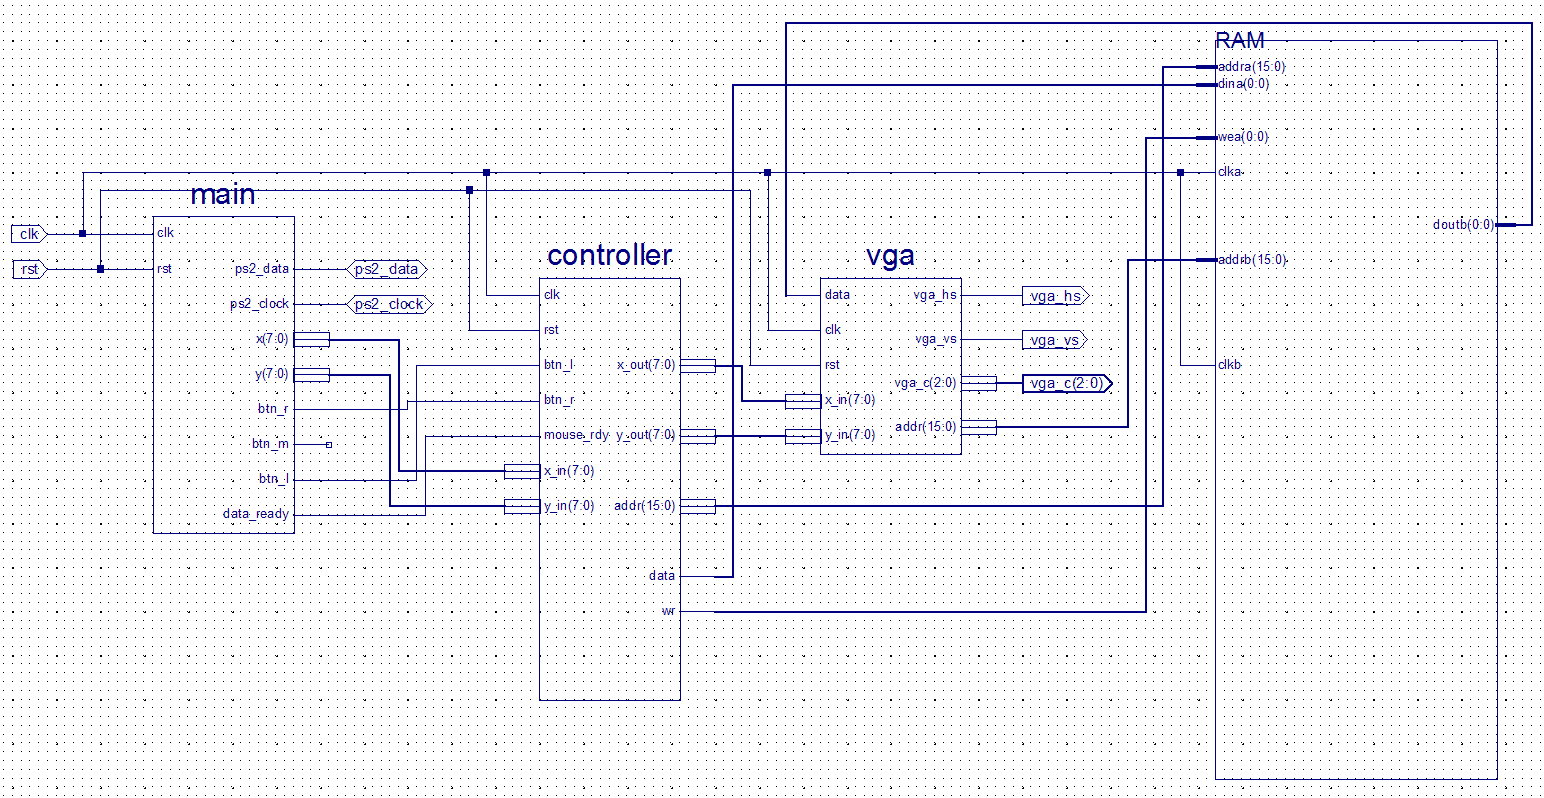
\includegraphics[scale=.45]{main.png}
\caption{Moduł \texttt{mouse\_test.sch}.}
\label{fig:main}
\end{center}
\end{figure}
\end{landscape}
\newpage

\begin{figure}[h!]
\begin{center}
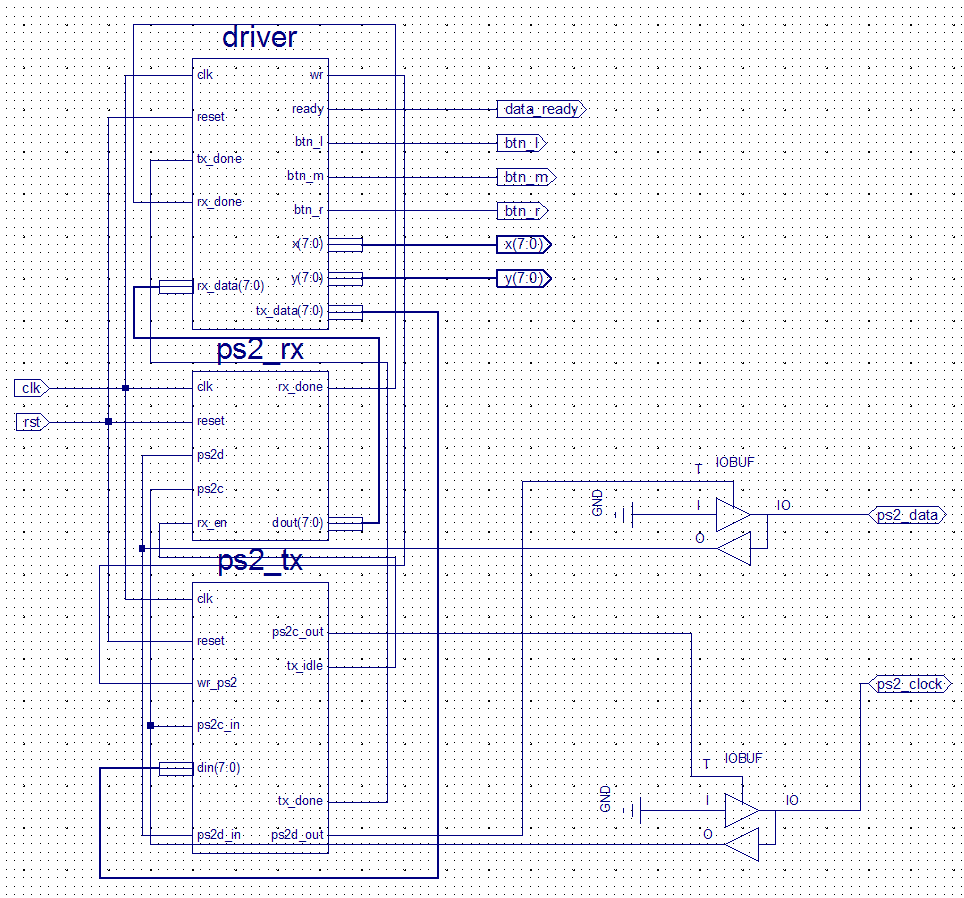
\includegraphics[scale=.45]{mouse.png}
\caption{Moduł \texttt{main.sch}.}
\label{fig:mouse}
\end{center}
\end{figure}

\subsection{Moduł \texttt{driver.vhd}}
Moduł ten odpowiada za inicjalizację oraz pobieranie informacji z myszy. Do tego
celu wykorzystuje moduły \texttt{ps2\_rx} oraz \texttt{ps2\_tx}.
Dane na wyjściach \texttt{x}, \texttt{y} i \texttt{btn\_*} są stabilne, gdy
sygnał \texttt{ready} ma wartość \texttt{1}. Moduł może znajdować się w jednym z
następujących stanów \texttt{init1} -- wysłanie bajtu inicjalizacji myszy,
\texttt{init2} -- oczekiwanie na koniec transmisji, \texttt{init3} --
oczekiwanie na bit potwierdzenia, \texttt{receive1}, \texttt{receive2},
\texttt{receive3} -- odbiór poszczególnych bajtów od myszy, \texttt{done} --
zakończenie transmisji od myszy.
\vspace{1em}

Sygnały wewnętrzne:
\begin{itemize}
  \item \texttt{state\_reg}, \texttt{state\_next} -- sygnał przechowujący stan
    układu
  \item \texttt{x\_reg(7:0)}, \texttt{x\_next(7:0)} -- sygnał zapisujący
    przesunięcie poziome
  \item \texttt{y\_reg(7:0)}, \texttt{y\_next(7:0)} -- sygnał zapisujący
    przesunięcie pionowe
  \item \texttt{btn\_reg(2:0)}, \texttt{btn\_next(2:0)} -- sygnał zapisujący
    stan przycisków myszy
\end{itemize}
\vspace{1em}
Wejścia:
\begin{itemize}
  \item \texttt{clk} -- zegar 50MHz
  \item \texttt{reset} -- reset układu
  \item \texttt{tx\_done} -- sygnał zakończenia nadawania
  \item \texttt{rx\_done} -- sygnał zakończenia odbioru
  \item \texttt{rx\_data(7:0)} -- dane odebrane od myszy
\end{itemize}
\vspace{1em}
Wyjścia:
\begin{itemize}
  \item \texttt{btn\_l} -- stan lewego przycisku myszy
  \item \texttt{btn\_m} -- stan środkowego przycisku myszy
  \item \texttt{btn\_r} -- stan prawego przycisku myszy
  \item \texttt{x(7:0)} -- przesunięcie poziome myszy
  \item \texttt{y(7:0)} -- przesunięcie pionowe myszy
  \item \texttt{ready} -- sygnał gotowości danych odebranych z myszy
  \item \texttt{tx\_data(7:0)} -- dane do wysłania do myszy
  \item \texttt{wr} -- sygnał rozpoczęcia wysyłania danych
\end{itemize}

\subsection{Moduł \texttt{ps2\_rx.vhd}}
Odbiornik danych z portu PS/2. Do wykrywania zbocza opadającego wykorzystywany
jest dwubitowy rejestr przesuwny. Dane na wyjściu są stabilne, gdy sygnał
\texttt{rx\_done} ma wartość \texttt{1}. Maszyna stanowa ma zaimplementowane
następujące stany \texttt{idle} -- oczekiwanie na transmisję, \texttt{busy} --
stan podczas transmisji, \texttt{done} -- koniec transmisji.
\vspace{1em}

Do modułu przygotowany został plik testowy, który symulował nadawanie bajtów
\texttt{0xF0}, \texttt{0x81} oraz \texttt{0xAA}.
Przebieg testowy dla modułu znajduje się na rysunku~\ref{fig:rx_test}.
\vspace{1em}

Sygnały wewnętrzne:
\begin{itemize}
  \item \texttt{state\_reg}, \texttt{state\_next} -- sygnał przechowujący stan
    układu
  \item \texttt{buf\_reg(10:0)}, \texttt{buf\_next(10:0)} -- bufor do zapisu
    danych
  \item \texttt{counter\_reg(3:0)}, \texttt{counter\_next(3:0)} -- licznik bitów
    do przesłania
  \item \texttt{fall\_edge} -- bit sygnalizujący wykrycie zbocza opadającego
  \item \texttt{ps2\_edge(2:0)} -- rejestr przesuwny dla wykrywacza zbocza
    opadającego
\end{itemize}
\vspace{1em}
Wejścia:
\begin{itemize}
  \item \texttt{clk} -- zegar 50MHz
  \item \texttt{reset} -- reset układu
  \item \texttt{ps2d} -- linia danych PS/2
  \item \texttt{ps2c} -- linia zegarowa PS/2
  \item \texttt{rx\_en} -- sygnał służący do włączenia odbiornika
\end{itemize}
\vspace{1em}
Wyjścia:
\begin{itemize}
  \item \texttt{rx\_done} -- sygnał gotowości danych odebranych z myszy
  \item \texttt{dout(7:0)} -- odebrany bajt
\end{itemize}

\subsection{Moduł \texttt{ps2\_tx.vhd}}
Nadajnik danych dla portu PS/2. Dla wykrywania zbocza opadającego wykorzystany
jest podobny mechanizm jak w module \texttt{ps2\_rx}. W maszynie stanowej
zaimplementowano następujące stany \texttt{idle} -- oczekiwanie na sygnał
rozpoczęcia transmisji, \texttt{rts} -- Request To Send, ściągnięcie linii
zegara na czas 100$\mu$s, \texttt{start} -- nadanie bitu startu, \texttt{data},
nadanie bitów danych oraz parzystości, \texttt{stop} -- koniec transmisji.
\vspace{1em}

Do modułu przygotowany został plik testowy, który symulował działanie urządzenia
podłączonego na magistralę PS/2, a nasz układ nadawał bajt \texttt{0xEE}.
Przebieg testowy dla modułu znajduje się na rysunku~\ref{fig:mouse_test}.
\vspace{1em}

Sygnały wewnętrzne:
\begin{itemize}
  \item \texttt{state\_reg}, \texttt{state\_next} -- sygnał przechowujący stan
    układu
  \item \texttt{buf\_reg(8:0)}, \texttt{buf\_next(8:0)} -- z danymi do wysłania
  \item \texttt{counter\_reg(3:0)}, \texttt{counter\_next(3:0)} -- licznik bitów
    do przesłania
  \item \texttt{rtsc\_reg(3:0)}, \texttt{rtsc\_next(3:0)} -- licznik czasu
    oczekiwania podczas stanu \texttt{rts}
  \item \texttt{parity} -- bit parzystości
  \item \texttt{fall\_edge} -- bit sygnalizujący wykrycie zbocza opadającego
  \item \texttt{ps2\_edge(2:0)} -- rejestr przesuwny dla wykrywacza zbocza
    opadającego
\end{itemize}
\vspace{1em}
Wejścia:
\begin{itemize}
  \item \texttt{clk} -- zegar 50MHz
  \item \texttt{reset} -- reset układu
  \item \texttt{ps2d\_in} -- linia danych PS/2
  \item \texttt{ps2c\_in} -- linia zegarowa PS/2
  \item \texttt{wr\_ps2} -- sygnał rozpoczęcia wysyłania
  \item \texttt{din(7:0)} -- bajt do wysłania
\end{itemize}
\vspace{1em}
Wyjścia:
\begin{itemize}
  \item \texttt{tx\_done} -- sygnał zakończenia nadawania
  \item \texttt{tx\_idle} -- sygnał bezczynności
  \item \texttt{ps2d\_out} -- linia danych PS/2
  \item \texttt{ps2c\_out} -- linia zegarowa PS/2
\end{itemize}

\subsection{Moduł \texttt{controller.vhd}}
Moduł interpretuje dane przychodzące z myszy, aktualizuje położenie kursora na
ekranie i odpowiada za zapisywanie danych do pamięci RAM. Jako jeden z
nielicznych modułów w VHDL nie został zaimplementowany jako maszyna stanowa.
\vspace{1em}

Sygnały wewnętrzne:
\begin{itemize}
  \item \texttt{pos\_x(7:0)}, \texttt{pos\_y(7:0)} -- rejestr zapisujący pozycję kursora
\end{itemize}
\vspace{1em}
Wejścia:
\begin{itemize}
  \item \texttt{clk} -- zegar 50MHz
  \item \texttt{rst} -- reset układu
  \item \texttt{btn\_l} -- stan lewego przycisku myszy
  \item \texttt{btn\_r} -- stan prawego przycisku myszy
  \item \texttt{mouse\_rdy} -- sygnał gotowości danych przychodzących
  \item \texttt{x\_in(7:0)} -- przesunięcie myszy w poziomie
  \item \texttt{y\_in(7:0)} -- przesunięcie myszy w pionie
\end{itemize}
\vspace{1em}
Wyjścia:
\begin{itemize}
  \item \texttt{data} -- bit danych do zapisu
  \item \texttt{wr} -- sygnał umożliwiający zapis do pamięci
  \item \texttt{addr(15:0)} -- adres do zapisu w pamięci
  \item \texttt{x\_out(7:0)} -- pozycja kursora w poziomie
  \item \texttt{y\_out(7:0)} -- pozycja kursora w pionie
\end{itemize}

\subsection{Moduł \texttt{vga.vhd}}
Moduł odpowiada za wyświetlanie grafiki zapisanej w pamięci RAM oraz pozycji
kursora. Aby uzyskać częstotliwość 25MHz zaimplementowany został dzielnik
częstotliwości 50MHz.
Jest to drugi moduł, który nie jest zaimplementowany jako maszyna stanowa.
\vspace{1em}

Sygnały wewnętrzne:
\begin{itemize}
  \item \texttt{clk\_25} -- zegar 25MHz
  \item \texttt{addr\_h(7:0)}, \texttt{addr\_v(7:0)} -- liczniki adresu w pionie
    i poziomie
  \item \texttt{ctr\_h(9:0)}, \texttt{ctr\_v(9:0)} -- liczniki dla generacji
    sygnałów synchronizacji
  \item \texttt{x}, \texttt{y} -- sygnały ułatwiające obliczanie pozycji kursora
\end{itemize}
\vspace{1em}
Wejścia:
\begin{itemize}
  \item \texttt{clk} -- zegar 50MHz
  \item \texttt{rst} -- reset układu
  \item \texttt{x\_in(7:0)} -- pozycja kursora w poziomie
  \item \texttt{y\_in(7:0)} -- pozycja kursora w pionie
  \item \texttt{data} -- odczytany bit z pamięci RAM
\end{itemize}
\vspace{1em}
Wyjścia:
\begin{itemize}
  \item \texttt{addr(15:0)} -- adres do odczytu z pamięci
  \item \texttt{vga\_vs} -- sygnał synchronizacji pionowej VGA
  \item \texttt{vga\_hs} -- sygnał synchronizacji poziomej VGA
  \item \texttt{vga\_c(2:0)} -- magistrala przesyłająca bity koloru do VGA
\end{itemize}

\begin{figure}[h!]
\begin{center}
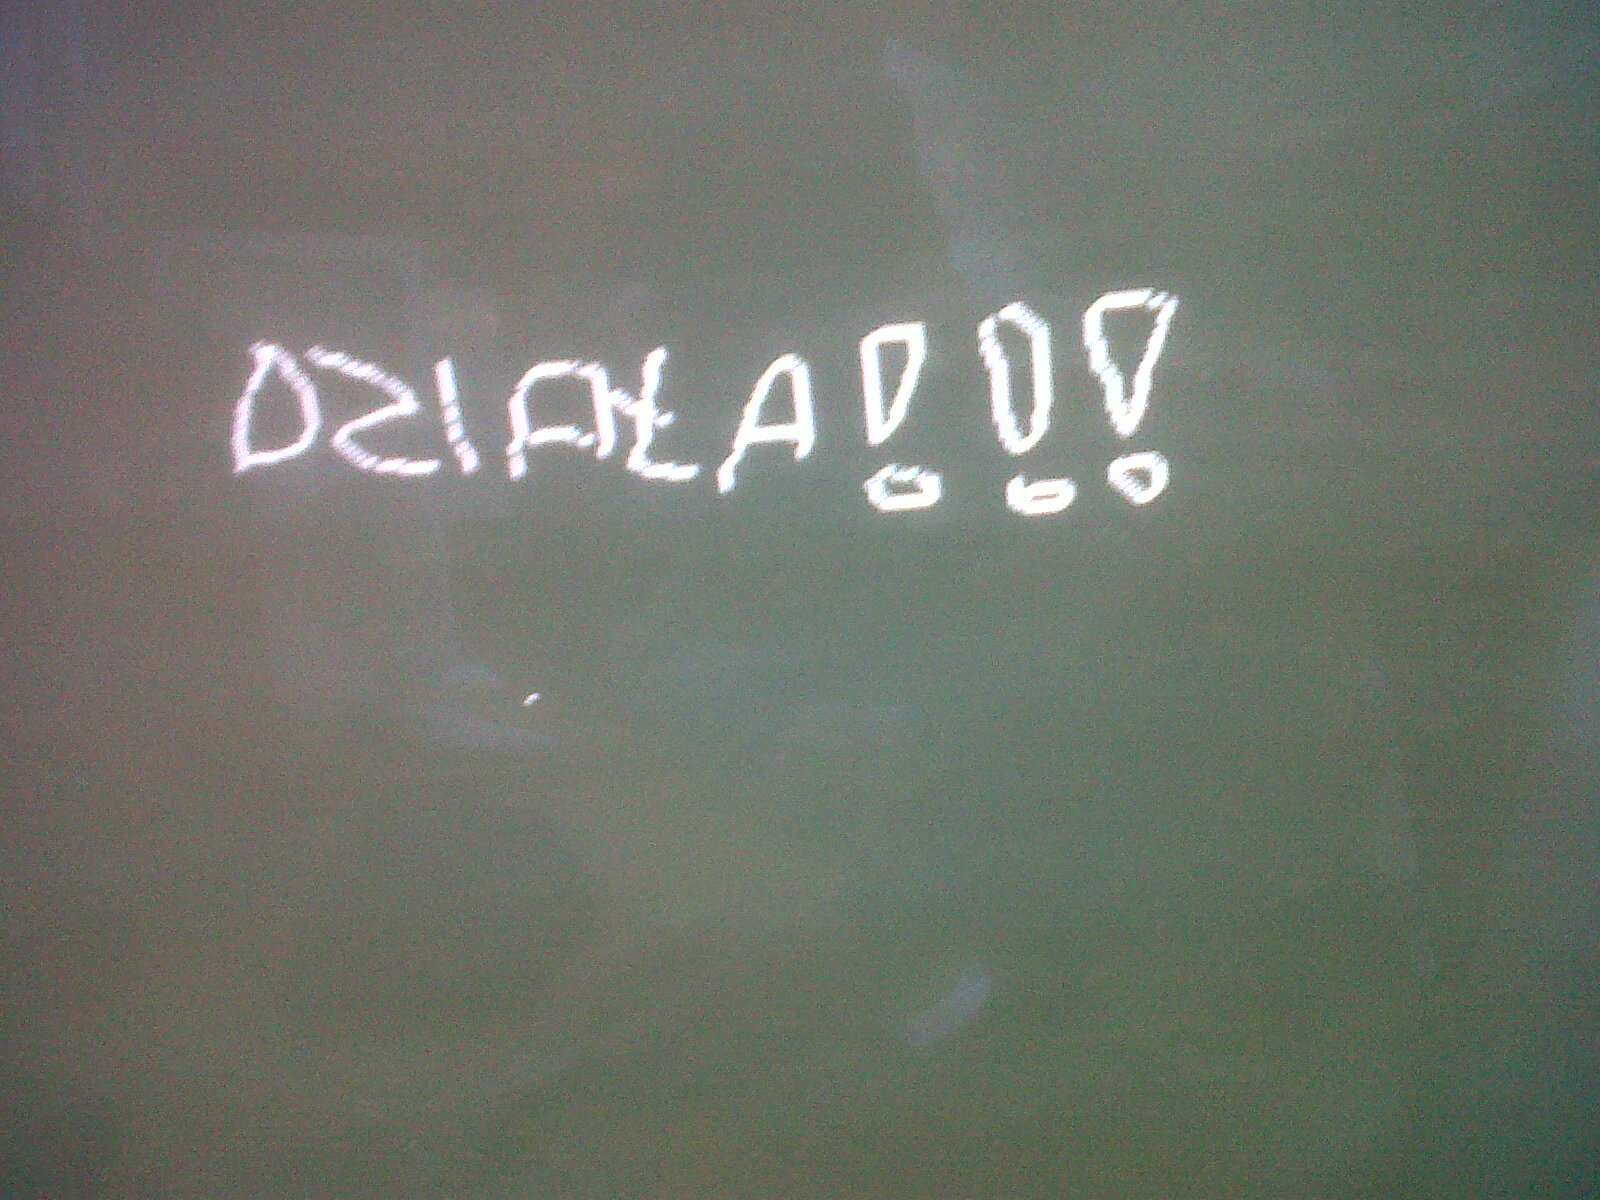
\includegraphics[scale=.3]{dziala.jpg}
\caption{Zdjęcie działającego układu.}
\label{fig:dziala}
\end{center}
\end{figure}

\newpage
\begin{landscape}
\begin{figure}[h!]
\begin{center}
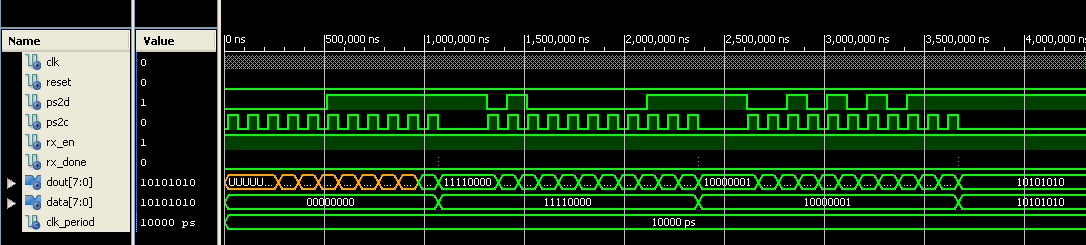
\includegraphics[scale=.6]{rx_test.png}
\caption{Przebieg testowy dla \texttt{ps2\_rx}.}
\label{fig:rx_test}
\end{center}
\end{figure}

\begin{figure}[h!]
\begin{center}
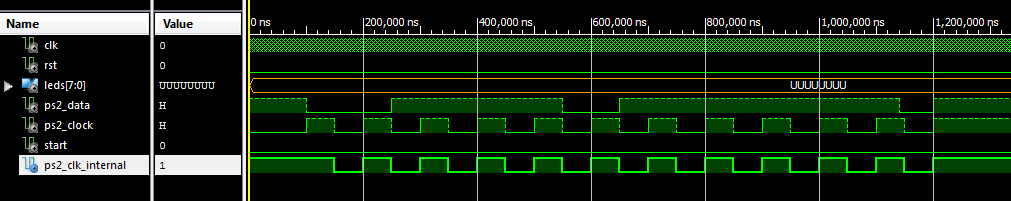
\includegraphics[scale=.85]{mouse_test.png}
\caption{Przebieg testowy dla modułu myszy.}
\label{fig:mouse_test}
\end{center}
\end{figure}
\end{landscape}
\newpage

\section{Wyniki syntezy}
\label{sec:synteza}

Podana przez syntezer szacowana maksymalna częstotliwość pracy układu wynosi
$145$MHz, więc jest około trzy razy większa niż częstotliwość, z którą ma
pracować układ. Tabela przedstawiająca zajętość zasobów znajduje się na
rysunku~\ref{fig:usage}. Zgodnie z przewidywaniami, układ na sprzęcie działa bez
zastrzeżeń.

\begin{figure}[h!]
\begin{center}
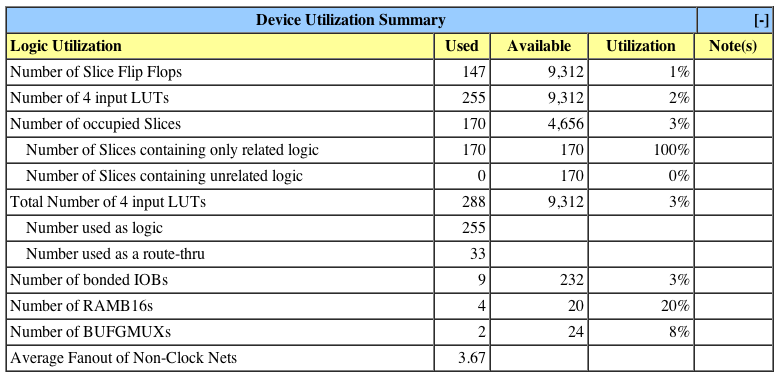
\includegraphics[scale=.6]{usage.png}
\caption{Użycie zasobów.}
\label{fig:usage}
\end{center}
\end{figure}


